\section{Introduction}
\label{sec:intro}

%\KZ{Our premise: Review sentences tend to be short and informative. It is our belief
%that every sentence in a review should provide some useful info.}

Abstractive opinion summarization is the process of 
producing a summary for a set of 
subjective user reviews given an entity 
(e.g., a place, a product, or a service). 
Such a set of reviews is called a {\em multi-review} in this paper. 
Deep learning (DL) techniques have made great successes 
in abstractive summarization
~\cite{NallapatiZSGX16,SeeLM17,LiuLZ18,CelikyilmazBHC18,BART20}, 
which requires training on a large number of document-summary pairs.
Unfortunately, the opinion summarization task 
generally lacks the multi-review and reference summary pairs,
as it is difficult for annotators to write summaries for 
multi-reviews on a large scale.

%\KZ{I still think the example in Table 1 is not that effective. I think
%the figure should highlight the main difference between our approach and the 
%previous approach to synthesize training data. And you better do it without using
%too many words but more like in a schematic. This example not only shows the
%diff between ours and their approach but also highlights the main advantage
%of this approach against others. I also don't understand the semicolons in the Ous part of the table. It's kind of messed up.}

Consequently, some approaches~\cite{MeanSum19,Copycat20,tree21}
adopt unsupervised learning, such as auto-encoder.
They are trained to reconstruct the encoding of individual reviews, which may prevent them from effectively reconstruct the aggregated encoding of multiple reviews for generating summary at test.
%but mainly focus on the content transformation within the multi-review of an entity.
%\KZ{What exactly is content transformation, and what's wrong with it?}
Other more popular approaches~\cite{Denoise20,Fewshot20,Plansum20,transsum21} 
focus on creating synthetic (multi-review, summary) pairs for training.
%\JQ{(multi-review,summary)}training data\JQ{pairs. delete: , which consists of multi-reviews and summaries.}
%Typical approaches sample some reviews from a set of reviews
%about an entity,  and treat them as summaries.
They typically sample one or more reviews from all reviews about an entity
%the multi-reivew
as ``pseudo'' summaries to use as the output of synthetic training pairs.
%Such methods have showed to outperform
%earlier auto-encoder models~\cite{MeanSum19,tree21} which requires no
%synthetic data. 
What sets them apart is the way in which input is created.
Existing approaches use either {\em textual} or  {\em structured} information.

%\begin{figure}[th]
%	\centering
%	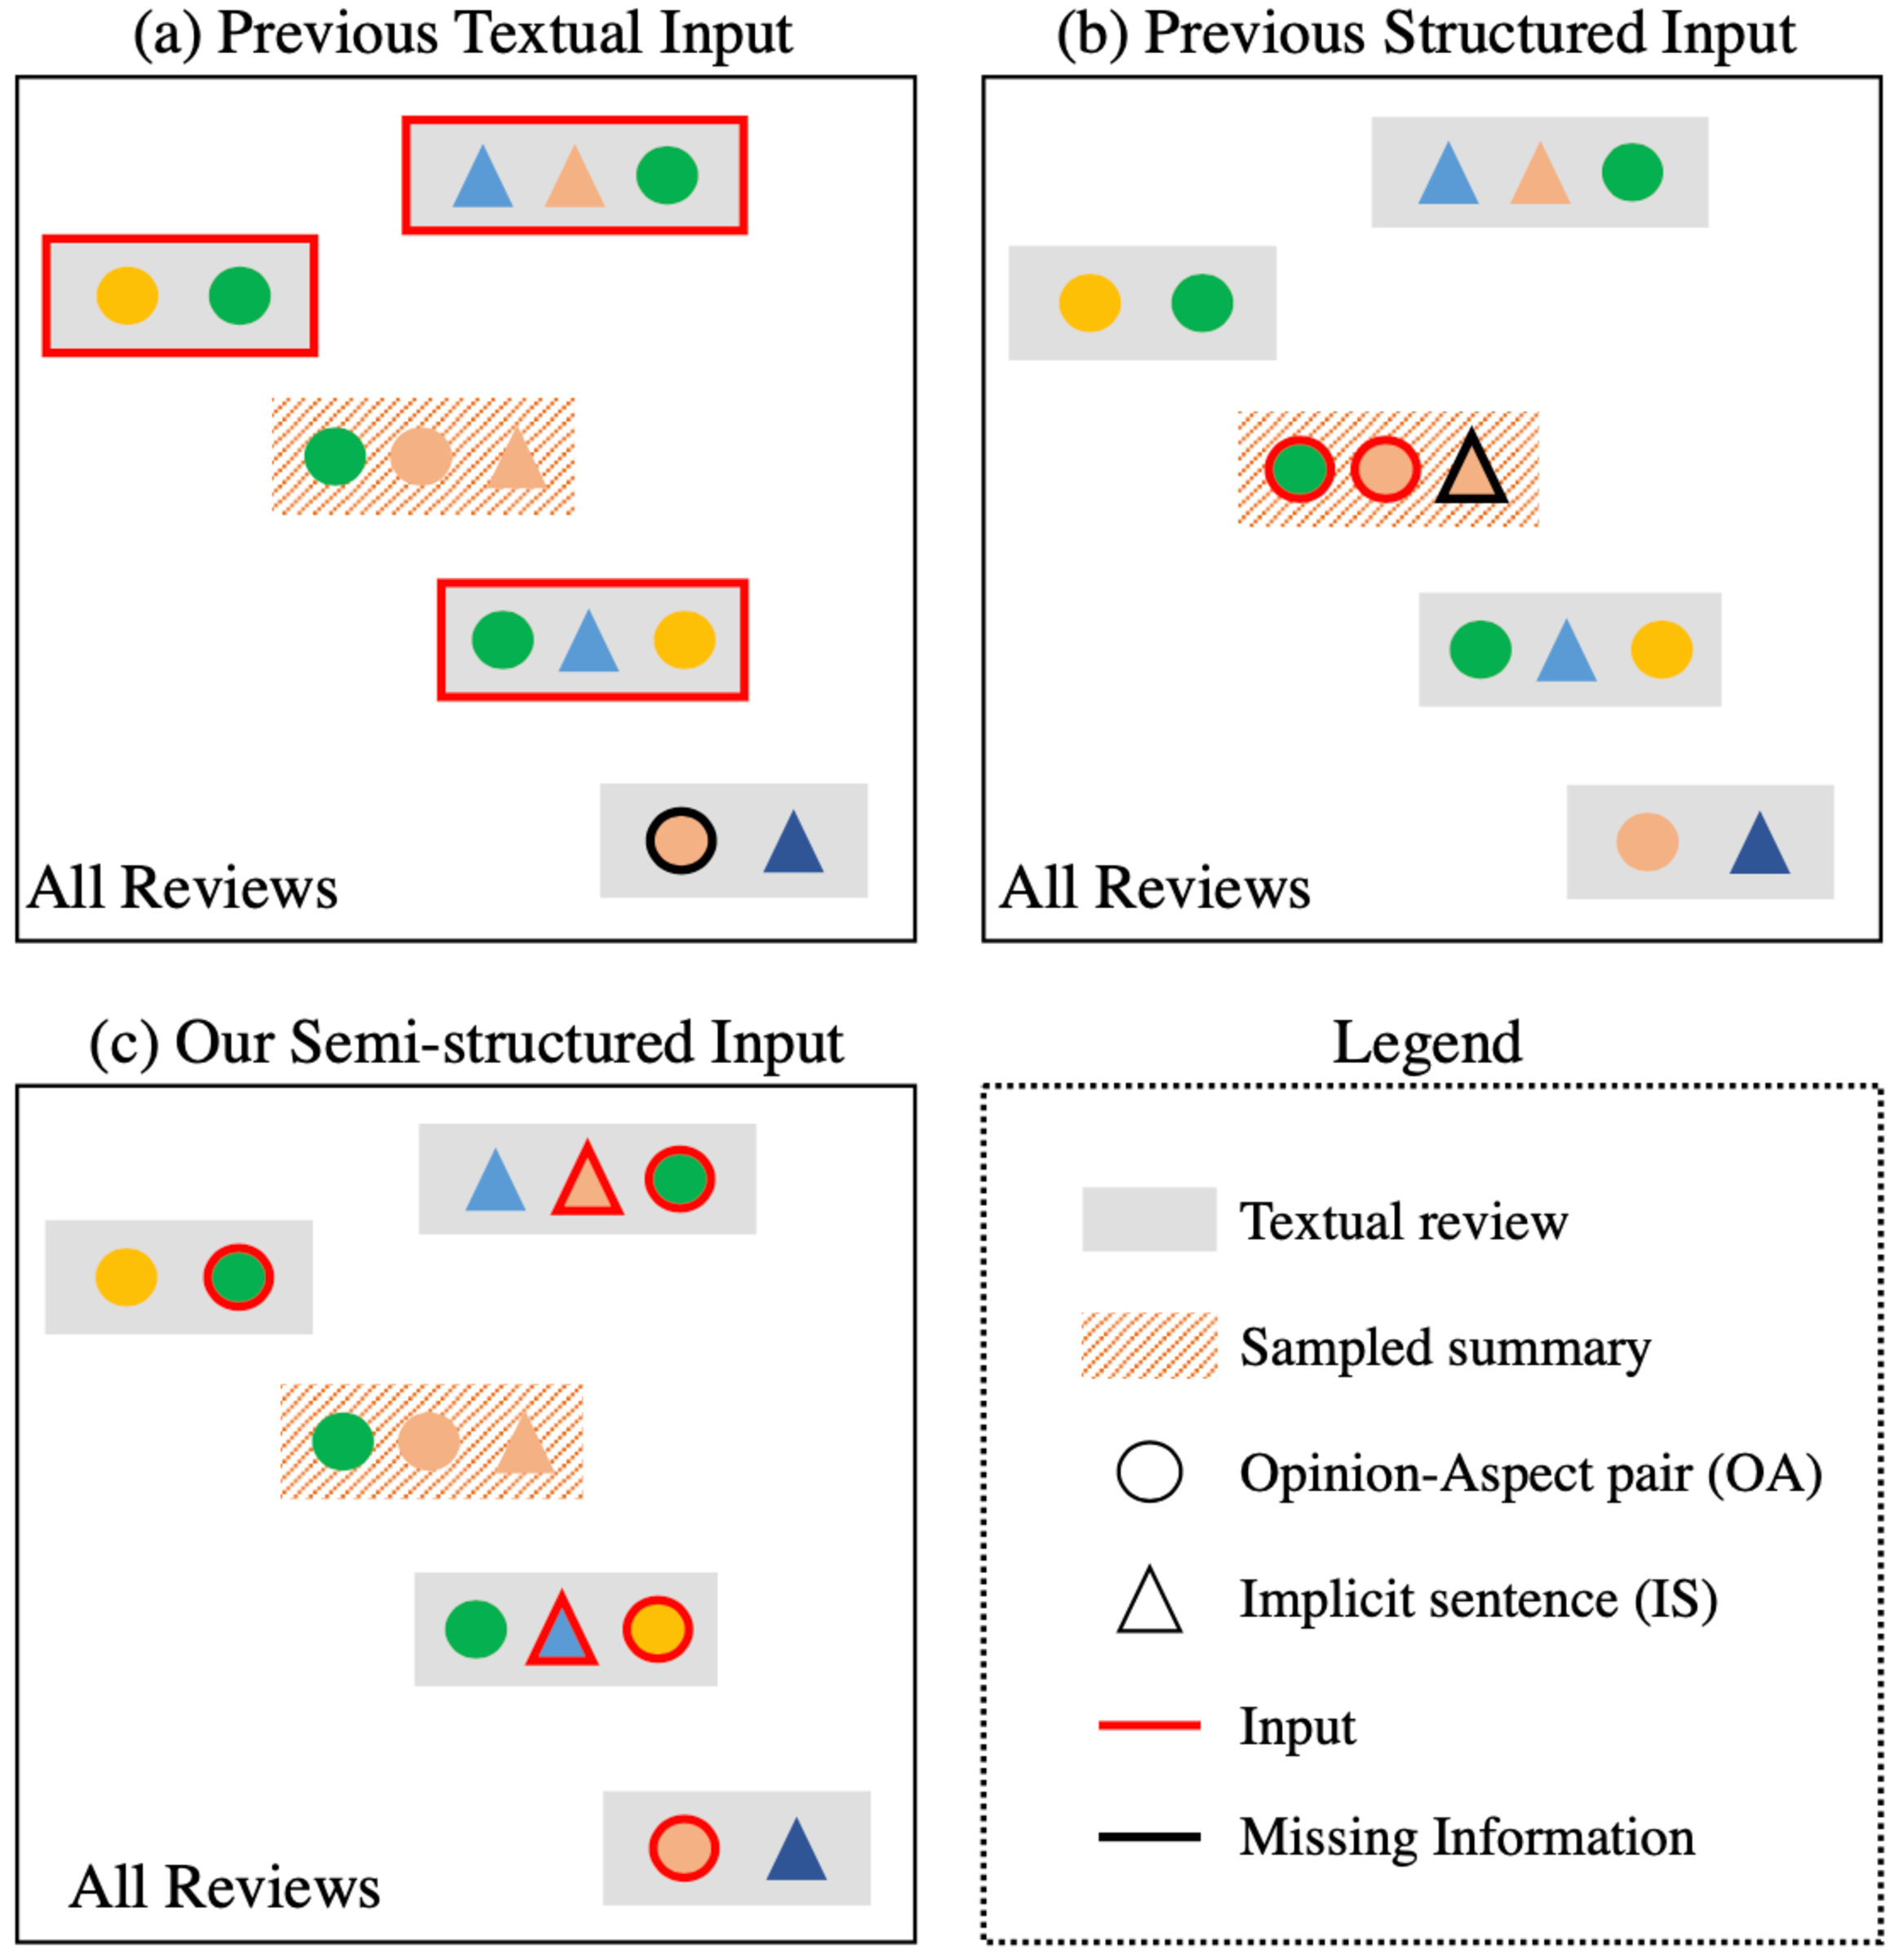
\includegraphics[width=0.85\linewidth]{./brief.pdf}
%	\caption{Different synthetic inputs of the same summary.
%	}
%	\label{fig:brief}
%\end{figure}


The {\em textual} input is usually a set of reviews sampled 
from the original multi-review. 
The most straight-forward method is {\em leave-one-out}~\cite{Copycat20}, 
which samples one review as summary and takes the rest as input. 
TranSum~\cite{transsum21} improves on {\em leave-one-out} by weighting 
each input review using its similarity to the summary.
However, these methods result in very long textual input, not only costing
more memory but also introducing some noises because the input of 
different summaries are almost identical except for one review.
An alternative to {\em leave-one-out} is to sample (or synthesize) several 
original reviews from all reviews, 
either randomly~\cite{Fewshot20}, or by the similarity between the input text and
the summary~\cite{Denoise20,Plansum20}.
%Their downside is that certain important information in the summary can be missing from the input such as ``beef'' (PlanSum and Denoise of \tabref{tab:previous_data}).
Their downsides are: i) the content of summary and its input may be completely unrelated  (FewSum of \tabref{tab:previous_data}); ii) certain important information in the summary can be missing from the input such as ``beef'' (PlanSum and Denoise of \tabref{tab:previous_data}).
%Their downsides is that certain important information in the summary can be missing from the input. As shown in \tabref{tab:previous_data}), the input of FewSum is completely unrelated to output. The input of PlanSum and Denoise miss ``beef''.
%\JQ{I don't think there are differences between these two downsides. Both means that there is information inconsistency between input and output. }

\begin{table}[th]
	\centering
	\scriptsize
	\begin{tabular}{|p{7.8cm}|}
		\hline \rule{0pt}{10pt}
		\makecell[c]{\bf Output (Sampled Summary)} \\
		\hline
		very \textbf{disappointed} in \textbf{food} and \textbf{service} . the \textbf{beef} was \textbf{burned} . 
		\underline{the \textbf{staff} \textbf{dismissed} my comments .} 
		\vspace{0.2em}\\
		\hline
	\end{tabular}
	\begin{tabular}{|m{0.8cm}|m{0.3cm}<{\centering}|m{5.8cm}|}
		\hline
		\multicolumn{3}{|c|}{\rule{0pt}{10pt} \bf Input}  \\	
		\hline
		\multirow{3}{0.1cm}{FewSum} & $R_1$ & very average spanish \textbf{food} .
		\\
		\cline{2-3}
		& $R_2$ &definitely not a peruvian restaurant
		.
		\\
		\cline{2-3}
		& $R_3$ &love this place! location is great
		.
		\\
		\hline
		\multirow{3}{0.1cm}{Denoise} & $R_1$ & very uncomfortable in \textbf{food} and \textbf{staff} . the \textbf{ food} was bad . the \textbf{staff} ignored me .
		\\
		\cline{2-3}
		& $R_2$ & bad \textbf{food} . the \textbf{staff} ignored me . very uncomfortable in restaurant .\\
		\cline{2-3}
		& $R_3$ &I was \textbf{disappointed} with the restaurant. the \textbf{food} was not bad . but the \textbf{staff} was unfriendly .
		\\
		\hline
		\multirow{3}{0.1cm}{PlanSum} & $R_1$ & bad \textbf{food} and \textbf{service} . \textbf{disappointed} \\
		\cline{2-3}
		& $R_2$& the \textbf{food} and \textbf{service} was not good . very \textbf{bad experience} .
		\\
		\cline{2-3}
		& $R_3$ &awful \textbf{food} and \textbf{service} . the \textbf{staff} was unfriendly .
		\\
		\hline
		OpiDig & OA & \textbf{disappointed}, \textbf{food; disappointed}, \textbf{service; burned}, \textbf{beef}
		\\
		\hline
		\multirow{2}{0.1cm}{Ours} & OA &not good, \textbf{food;} great, location\textbf{;} bad, \textbf{food; disappointed}, \textbf{service;} not fresh, \textbf{beef;} unfriendly, \textbf{staff;} awful, \textbf{service}\\
		\cline{2-3}
		& IS &not recommended\textbf{;} my questions were \textbf{dismissed} .\textbf{;} the \textbf{staff} ignored our \textbf{comments} .\\
		\hline
	\end{tabular}
	\caption{The synthetic training pairs (Input, Output) with the same summary 
		by different methods. The underlined sentences don't contain explicit opinion-aspect pairs (OA), 
		which are called ``implicit sentences'' (IS).  
		%$R$ is textual review, OA is opinion-aspect pair and IS is implicit sentence. 
		Bolded words in the input and output are matched.
		``;'' delimits OAs and ISs in our method.
	}\label{tab:previous_data}  
\end{table}


It is widely acknowledged that when summarizing reviews, the most critical information
to be considered are 
aspects of the product or service that appear in the reviews,
%aspects of the product or service,
and opinions about these aspects~\cite{AngelidisL18,MukherjeePVGBG20}.
Hence it is natural to consider extracting the {\em structured} information, 
that is, opinion-aspect pairs (OAs) such as (burned, beef) and (disappointed, service) 
from reviews first, and then doing summarization.
%It ignores the implicit sentences (ISs), which are the sentences cannot extract typical OA pairs, as shown in \figref{fig:brief}(b).
%\YZ{Add Quantitive analysis for OA and IS}
OpiDig~\cite{OpiDig20} adopts a self-supervised approach, and uses a review as output 
and extracts OAs from this review as input with a self-training seq2seq model.
At testing, OpiDig clusters the OAs 
of multi-reviews and selects those pairs in the center as input to 
generate a summary. 
Due to the inherent weakness of OA pair extraction algorithms, %and linguistic challenges, 
%some aspects or opinions can't be easily extracted,
%e.g., ``staff'' in \tabref{tab:previous_data}. 
some sentences can't easily extract pairs of opinion and aspect,
e.g., the sentence about ``staff'' in \tabref{tab:previous_data}. 
We call these sentences ``implicit sentences'' (ISs).
%\JQ{due to the imperfect extractor? }
%The generated summary can only make sentences according 
%to the selected OAs and also suffers from the noising inherent to clustering.
%\JQ{Previous methods can be merged into one paragraph, quite detailed and may be explained in Related work.}

%\KZ{Combined the following three paras into one
%and shorten it significantly. Focus on the motivation
%of your approach by observing the example, not talking
%about the details of the approach. Leave the details
%to the approach section. Only briefly mentioning the solution
%using a sentence or two.}
\cut{%%%
In this paper, we tackle the pitfalls of the previous
work by using semi-structured data instead of 
only {\em textual} input (free multi-reviews )
or only {\em structured }input (opinion-aspect pairs) as training data. 
We create synthetic training data by 
sampling some reviews as summaries first.
The sampled summaries resemble 
the human-written summaries of multi-reviews in writing style.
As opinion and aspect are the most important for opinion summarization,
we directly extract OAs from summary
to generate input.
As shown in \figref{fig:example},
the aspects in multi-review are the noisy version of the aspects in summary.
Therefore, we generate noisy OAs for summary by
extracting appropriate OAs from reviews under the 
same entity with summary, 
which simulates the OAs in actual multi-review.

However, 
using OAs as input alone ignores some useful information,
such as the orange sentences in \figref{fig:example}.
As the reviews tend to be short and informative,
it is our belief that every sentence in a review should provide some useful information.
During actual multi-review summarization,
some specific information in summary
is abstracted from some sentences without OAs in multi-review.
Thus, we collect the sentences that cannot extract OAs in summary as implicit sentences (IS's),
and generate the noisy version by sampling sentences from 
multi-review. 
%The synthetic dataset with OAs and ISs as input 
%points out the OAs which is the most salience information in opinion summarization.
%Meanwhile, ISs can help reducing the loss of information.
}%%%%

With the lessons learned from previous approaches,
in this paper, we propose to use semi-structured data, 
instead of only textual or structured multi-reviews as the input of our synthetic
training data. 
For a review, its OAs express the opinion explicitly
and ISs express the opinion implicitly through the description of specific information.
As reviews tend to be short and informative,
we believe that every sentence in them provides some useful information and should not be neglected.
%\JQ{delete: Reviews reflect the users' opinion of the entities and have 
%special writting style.}
%OAs, as \textit{explicit information},
%are always the most important for reviews.
%However,
%according to previous methods, using OAs to represent a review alone ignores some \textit{specific information},
%such as the sentences about the ``staff'' in \tabref{tab:previous_data}.
To this end, our semi-structured input is a combination of OAs and ISs.
%Given a review as the output of training pair, 
%we extract opinion-aspect pairs (OAs) from sampled summary
%to generate the input.
%However, as shown in \tabref{tab:previous_data},
%some sentences that reflect the details in review don't have typical OAs. 
%Thus, for each review, we also collect the sentences that cannot extract OAs as implicit sentences (ISs).
%In this way, the review can be represented in the semi-structured format with OAs and ISs,
%as shown in \figref{fig:brief}.

%\KZ{Please rewrite this paragraph. I don't understand what you are talking about!}
We create a synthetic training data by 
first sampling a textual review as ``pseudo'' summary.
Since in the actual opinion summarization scenario,
OAs and ISs in a multi-review contain redundancies and contradictories comparing with them in the summary.
To simulate this reality, we construct the noisy version of OAs and ISs in a ``pseudo'' summary as the corresponding multi-review 
by sampling OAs and ISs from all reviews under the same entity except the ``pseudo'' summary.
%the OAs and ISs of multi-review are the noisy version of .
% which contains the many OAs and ISs consistent with summary and some redundant OAs and ISs.
%For a ``pseudo'' summary under an entity, we sample OAs and ISs from
%all reviews under the same entity according OAs and ISs of the summary to simulate noisy OAs and ISs in the actual multi-review.
%The sampled OAs and ISs is the noisy version of them in summary.
As shown in \tabref{tab:previous_data}, 
compared with taking multiple textual 
reviews or OAs extracted from a single review as input,
our noisy OAs and ISs %selected from all reviews 
reduce the probability that the summary can't be abstracted from the synthetic input,
and help model learn to attend to salient aspects and opinions.
%weaken the information inconsistency between synthetic multi-review and summary.
%\JQ{here we allow the existence of inconsistency, why the inconsistency is a weakness in previous method?}
%\JQ{delete: As shown in \tabref{tab:previous_data},
%some information of the summary cannot be summarized
%from the multiple textual reviews or OAs extracted from single review as input,
%such as ``the beef was burned''.}

%For a review, its OAs express the opinion explicity
%and the ISs without OAs express the opinion implicitly through the description of specific information.
In order to capture explicit opinion (opinion-aspect pairs) 
and implicit opinion (implicit sentences) at same time,
%\KZ{I don't understand why OA pairs are generalized and why IS are specific. Need to explain this.}
we propose an aspect-guided model with an OA encoder and
an IS encoder. %sharing parameters. 
We first train a single encoder model variation by taking only noisy OAs as input. 
Then, we initialize our dual encoder model with this pretrained model and take both OAs and ISs as input.
In this way, our model not only allows the information of OA and IS to 
complement each other but also generates summaries with less information missing.%which avoids missing information in the generated summary.
%Better results can be obtained by 
%training on basic model first and then fine-tuning on modified model.
%As shown in \tabref{tab:example}, 
%the summary generated by modified model is more informative.
%Because the pretrained basic model can provides
%the main aspects and its opinion for summary and
%the modified model help supplement specific information.
%\JQ{ We do not simply concatenate noisy OAs and ISs as input since we need expand some important pairs in noisy OAs into sentences and abstract noisy ISs.}\JQ{do not understand, or explain in approach.}
%the noisy OAs need 
%but noisy ISs need abstraction. 
%More details are shown in \secref{sec:results}.

In summary, our contributions are as follows:
\begin{enumerate}
\item We find that semi-structured synthetic dataset,
which uses OAs and ISs as input 
and textual summary as output, 
is more effective than the synthetic dataset using only textual reviews or only OAs as input.
%\KZ{We need a better word for ``other sentence''
%so people can understand immediately.}
%We show that this is more effective than relying on
%only textual reviews or only opinion-aspect pairs in previous work. 
(\tabref{tab:traindata})

%\item We propose aspect-variant guided models to deal with
%opinion-aspect pairs and other sentences. (\secref{sec:model}) 
\item 
We propose a new data creation method to obtain
%approach for opinion summarization,
%which first creates 
semi-structured synthetic training pairs by sampling the noisy version of 
OAs and ISs as the input together with an aspect-guided model with dual encoder. %for such data.
%consisting of
%opinion-aspect encoder and implicit sentence encoder.
(\secref{sec:approach})

\item 
%Our semi-structured synthetic training data is more effective than the training data 
%relying completely on text or opinion-aspect pairs in previous work. 
Compared with previous opinion summarization systems, 
the proposed model trained on our synthetic dataset substantially outperforms the 
state-of-the-art methods on the Yelp and Amazon datasets. (\tabref{tab:all})
\end{enumerate}
